\documentclass[aspectratio=169, 12pt]{beamer}

% ── Theme & colors ──────────────────────────────────────────────
\usetheme{Madrid}
\usecolortheme{seahorse}
\setbeamertemplate{navigation symbols}{}
\setbeamertemplate{footline}[frame number]

\usepackage{amsmath, amssymb, bm}
\usepackage{graphicx}
\usepackage{booktabs}
\usepackage{tikz}
\usetikzlibrary{arrows.meta, positioning, calc}

\newcommand{\R}{\mathbb{R}}
\newcommand{\Rcd}{R_{\mathrm{cd}}}
\newcommand{\tcd}{\mathbf{t}_{\mathrm{cd}}}
\newcommand{\Rdc}{R_{\mathrm{dc}}}
\newcommand{\tdc}{\mathbf{t}_{\mathrm{dc}}}
\newcommand{\skewmat}[1]{\left[#1\right]_{\times}}
\newcommand{\norm}[1]{\left\lVert #1 \right\rVert}

\title{Cost-Effective Domain Adaptation via\\Rail Motion-Manifold Self-Supervision}
\subtitle{Adapting XFeat with Circular \& Linear Rail Priors --- No Labels Required}
\author{Shantnu}
\date{\today}

\begin{document}

% ================================================================
%  TITLE
% ================================================================
\begin{frame}
\titlepage
\end{frame}

% ================================================================
%  OUTLINE
% ================================================================
\begin{frame}{Outline}
\tableofcontents
\end{frame}

% ================================================================
\section{Motivation \& High-Level Idea}
% ================================================================

\begin{frame}{The Challenge: Domain Gap in Feature Matching}
\small
\begin{itemize}\setlength{\itemsep}{3pt}
    \item Off-the-shelf feature matchers (XFeat, SuperPoint, etc.) are trained on
          large-scale internet photo collections (MegaDepth) and synthetic warps.
    \item In \textbf{target deployment domains} these models can degrade due to:
    \begin{itemize}\setlength{\itemsep}{1pt}
        \item \textbf{Challenging lighting} --- low light, specular highlights, harsh shadows.
        \item \textbf{Low / repetitive texture} --- industrial parts, walls, floors.
        \item \textbf{Motion blur} --- fast-moving cameras or conveyor systems.
        \item \textbf{Domain-specific appearance} --- medical, agricultural, manufacturing scenes
              rarely seen in training data.
    \end{itemize}
    \item \textbf{Result:} Fewer correct matches $\Rightarrow$ degraded pose estimation,
          SLAM drift, inspection failures.
\end{itemize}
\end{frame}

% ================================================================
\begin{frame}{Our Approach: Labels Are Expensive, Rails Are Cheap}
\small
\begin{columns}[T]
\column{0.52\textwidth}
\textbf{What we do NOT have:}
\begin{itemize}\setlength{\itemsep}{2pt}
    \item[$\times$] Ground-truth correspondences for the target domain.
    \item[$\times$] Motion-capture or encoder-based pose labels.
    \item[$\times$] Large labeled datasets of the deployment scene.
\end{itemize}

\smallskip
\textbf{What we DO have:}
\begin{itemize}\setlength{\itemsep}{2pt}
    \item[$\checkmark$] A \textbf{mechanical rail} (circular or linear) used during data collection.
    \item[$\checkmark$] Camera \textbf{intrinsics} $K$ (from calibration).
    \item[$\checkmark$] Camera-to-device \textbf{extrinsics} $(R_{\mathrm{cd}}, \mathbf{t}_{\mathrm{cd}})$.
\end{itemize}

\column{0.45\textwidth}
\textbf{Key idea:}
\begin{enumerate}\setlength{\itemsep}{2pt}
    \item The rail constrains camera motion to a \textbf{known 1D manifold}.
    \item This gives us a \textbf{free geometric supervision signal}:
          matches must satisfy an epipolar constraint parameterized by a single scalar.
    \item We use this to \textbf{fine-tune} XFeat on the target domain ---
          no labels, no mocap, no encoders.
\end{enumerate}
\end{columns}

\vspace{0.3em}
\begin{center}
\fbox{\parbox{0.85\textwidth}{\centering
\textbf{Goal:} Adapt XFeat so predicted correspondences are more consistent with
the target domain, while preserving generalization from the original training.
}}
\end{center}
\end{frame}

% ================================================================
\begin{frame}{Why This Is Cost-Effective}
\small
\begin{center}
\begin{tabular}{lcc}
\toprule
\textbf{Supervision source} & \textbf{Cost / effort} & \textbf{Domain-specific?} \\
\midrule
MegaDepth (internet photos) & Free (public dataset) & No (generic) \\
Synthetic homographies & Cheap (augmentation) & No (generic) \\
Motion capture / encoders & \$\$\$ (hardware + setup) & Yes \\
Manual correspondences & \$\$\$ (human annotation) & Yes \\
\midrule
\textbf{Rail manifold prior} & \textbf{\$ (off-the-shelf rail)} & \textbf{Yes} \\
\bottomrule
\end{tabular}
\end{center}

\vspace{0.3em}
\begin{itemize}\setlength{\itemsep}{2pt}
    \item Rails / sliders are standard, inexpensive mechanical components.
    \item A single image pair from the rail is enough to define the loss.
    \item The geometric constraint is \textbf{exact} (up to calibration accuracy) --- no label noise.
\end{itemize}
\end{frame}

% ================================================================
\begin{frame}{Why Self-Supervise on a Known Motion Manifold?}
\small
\begin{itemize}\setlength{\itemsep}{4pt}
    \item \textbf{Problem:} Standard XFeat training uses MegaDepth / synthetic homographies.
          These provide \emph{generic} correspondence supervision, but no domain-specific geometric signal.
    \item \textbf{Opportunity:} In many real deployment scenarios the camera moves on a
          \emph{known mechanical manifold} (e.g.\ a circular rail or a linear slider).
    \item \textbf{Key insight:} If we know the manifold, the \emph{epipolar geometry}
          between any two views is fully determined by a \textbf{single scalar parameter}
          (angle $\phi$ for circular, sign $s$ for linear).
    \item \textbf{Goal:} Add a \emph{self-supervision loss} that rewards the network for
          producing matches whose epipolar residuals are consistent with the known manifold geometry.
\end{itemize}
\end{frame}

% ================================================================
\begin{frame}{What Changes in the Training Pipeline?}
\small
\begin{enumerate}\setlength{\itemsep}{3pt}
    \item A \textbf{fixed image pair} from the rail is loaded at init (resized, grayscale).
    \item Every training step, the network also processes this pair $\rightarrow$ features + heatmaps.
    \item \textbf{Matches are extracted} (top-$k$ mutual nearest neighbors in descriptor space).
    \item A \textbf{rail loss} measures how well those matches satisfy the epipolar constraint
          on the known manifold.
    \item The rail loss is added to the standard XFeat loss with weight $\lambda_{\mathrm{rail}}$.
\end{enumerate}

\vspace{0.3em}
\textbf{No additional ground-truth labels are needed} --- only the camera intrinsics $K_0, K_1$
and the camera-to-device extrinsics $(\Rcd, \tcd)$.
\end{frame}

% ================================================================
\section{Coordinate Systems \& Extrinsics Convention}
% ================================================================

\begin{frame}{Coordinate Frames}
\small
\begin{columns}[T]
\column{0.55\textwidth}
We define two frames:
\begin{itemize}\setlength{\itemsep}{2pt}
    \item \textbf{Camera frame} --- the standard pinhole camera coordinate system
          (origin at optical center, $Z$ forward, $X$ right, $Y$ down).
    \item \textbf{Device frame} --- attached to the physical rig/slider. The manifold
          motion (rotation or translation) is described in this frame.
\end{itemize}

\smallskip
\textbf{Extrinsics convention (camera $\to$ device):}
\[
    \mathbf{p}_{\mathrm{dev}} = \Rcd \, \mathbf{p}_{\mathrm{cam}} + \tcd
\]

\column{0.42\textwidth}
\begin{center}
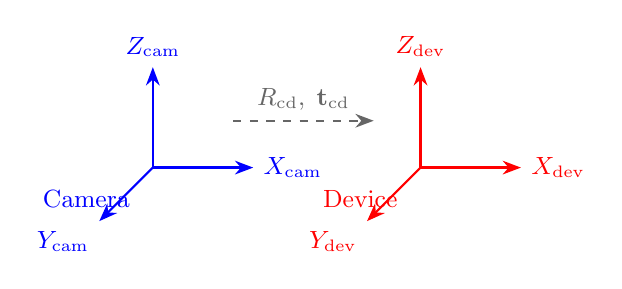
\begin{tikzpicture}[>=Stealth, scale=0.85, every node/.style={font=\small}]
  % Camera frame
  \draw[->, thick, blue] (0,0) -- (1.5,0) node[right]{$X_{\mathrm{cam}}$};
  \draw[->, thick, blue] (0,0) -- (0,1.5) node[above]{$Z_{\mathrm{cam}}$};
  \draw[->, thick, blue] (0,0) -- (-0.8,-0.8) node[below left]{$Y_{\mathrm{cam}}$};
  \node[blue, anchor=north east] at (-0.2,-0.2) {Camera};

  % Device frame
  \draw[->, thick, red] (4,0) -- (5.5,0) node[right]{$X_{\mathrm{dev}}$};
  \draw[->, thick, red] (4,0) -- (4,1.5) node[above]{$Z_{\mathrm{dev}}$};
  \draw[->, thick, red] (4,0) -- (3.2,-0.8) node[below left]{$Y_{\mathrm{dev}}$};
  \node[red, anchor=north east] at (3.8,-0.2) {Device};

  % Arrow
  \draw[->, thick, dashed, black!60] (1.2,0.7) -- (3.3,0.7)
    node[midway, above]{$\Rcd,\;\tcd$};
\end{tikzpicture}
\end{center}
\end{columns}

\smallskip
Internally the code converts to \textbf{device $\to$ camera} when needed:
\vspace{-0.3em}
\[
    \Rdc = \Rcd^\top, \qquad \tdc = -\Rcd^\top \tcd
\]
\end{frame}

% ================================================================
\section{Geometry: Circular Rail}
% ================================================================

\begin{frame}{Circular Rail --- Physical Setup}
\small
\begin{itemize}\setlength{\itemsep}{2pt}
    \item The device moves on a \textbf{circle of radius $R$} in the device $XY$-plane,
          rotating about the device $Z$-axis.
    \item The reference position is at $\mathbf{p}_0 = [R,\; 0,\; 0]^\top$ in device coords.
    \item A second view is at angle $\phi$ away on the same circle.
    \item \textbf{Unknowns:} only $\phi$ (a single scalar).
\end{itemize}

\begin{center}
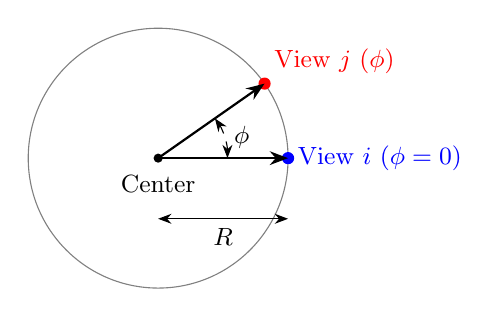
\begin{tikzpicture}[>=Stealth, scale=1.1]
  \draw[gray, thin] (0,0) circle(1.5);
  \fill[blue] (1.5,0) circle(2pt) node[right]{\small View $i$ ($\phi=0$)};
  \fill[red] ({1.5*cos(35)},{1.5*sin(35)}) circle(2pt)
    node[above right]{\small View $j$ ($\phi$)};
  \draw[->, thick] (0,0) -- (1.5,0);
  \draw[->, thick] (0,0) -- ({1.5*cos(35)},{1.5*sin(35)});
  \draw[<->, dashed] (0.8,0) arc(0:35:0.8) node[midway, right]{\small $\phi$};
  \node at (0,-0.3) {\small Center};
  \fill (0,0) circle(1.5pt);
  \draw[<->] (0,-0.7) -- (1.5,-0.7) node[midway, below]{\small $R$};
\end{tikzpicture}
\end{center}
\end{frame}

% ================================================================
\begin{frame}{Circular Rail --- Essential Matrix $E(\phi)$}
\small
The relative pose from view $i$ to view $j$ \textbf{in camera coordinates} is:
\vspace{-0.3em}
\[
    R_{ji} = \Rdc^\top \, R_z(-\phi) \, \Rdc
\]
\vspace{-1.2em}
\[
    \mathbf{t}_{ji} = \Rdc^\top \!\left(
        R_z(-\phi)\,\mathbf{p}_0 - \mathbf{p}_0
        + \bigl(R_z(-\phi) - I\bigr)\,\tdc
    \right)
\]
\vspace{-0.5em}
where $R_z(\theta)$ is the standard rotation about $Z$:
\vspace{-0.3em}
\[
    R_z(\theta) = \begin{pmatrix}
        \cos\theta & -\sin\theta & 0 \\
        \sin\theta &  \cos\theta & 0 \\
        0          &  0          & 1
    \end{pmatrix}
\]
\vspace{-0.5em}
The Essential matrix is then:
\vspace{-0.3em}
\[
    \boxed{E(\phi) = \skewmat{\mathbf{t}_{ji}} \, R_{ji}}
\]
\end{frame}

% ================================================================
\begin{frame}{Circular Rail --- Solving for $\phi^*$}
\small
We wrap each Sampson residual in a \textbf{Charbonnier kernel}
$\rho(r)=\sqrt{r+\varepsilon^{2}}$ --- a smooth, differentiable
approximation to $\sqrt{r}$ that is robust to outlier matches.

\smallskip
\textbf{Step 1 -- Coarse grid search} over $\phi\!\in\![\phi_{\min},\phi_{\max}]$:
\vspace{-0.5em}
\[
    J(\phi) \;=\; \sum_{m=1}^{M} w_m \;\rho\!\bigl(d_{\text{Sampson}}(\hat{\mathbf{x}}_m^{(1)},\,\hat{\mathbf{x}}_m^{(2)},\,E(\phi))\bigr)
\]
\vspace{-0.8em}

\noindent where $w_m$ are differentiable match weights and
$\hat{\mathbf{x}}^{(k)}\!=\!K^{-1}[u,v,1]^{\!\top}$.

\smallskip
\textbf{Step 2 -- Gauss--Newton refinement} (finite-difference Hessian):
\vspace{-0.5em}
\[
    g = \frac{J(\phi{+}\delta)-J(\phi{-}\delta)}{2\delta},\qquad
    H = \frac{J(\phi{+}\delta)-2J(\phi)+J(\phi{-}\delta)}{\delta^{2}}
\]
\vspace{-0.8em}
\[
    \phi \;\leftarrow\; \mathrm{clamp}\!\!\left(\phi - \tfrac{g}{H+10^{-6}},\;\phi_{\min},\;\phi_{\max}\right)
\]
\vspace{-0.5em}

\textbf{Key:} The solver runs under \texttt{torch.no\_grad()} (stop-grad).
Gradients flow only through $w_m$ and the final $J(\phi^{*})$.
\end{frame}

% ================================================================
\section{Geometry: Linear Rail}
% ================================================================

\begin{frame}{Linear Rail --- Physical Setup}
\small
\begin{itemize}\setlength{\itemsep}{2pt}
    \item The device translates \textbf{sideways along the device $+X$-axis} with \textbf{no rotation}.
    \item Orientation is fixed: $R_{ji} = I_{3\times 3}$.
    \item Translation direction in device frame:
          $\mathbf{t}_{\mathrm{dev}} \propto s \cdot [1,\; 0,\; 0]^\top$
          where $s \in \{+1, -1\}$.
    \item \textbf{Unknowns:} only the sign $s$ (or fixed to $+1$).
\end{itemize}

\begin{center}
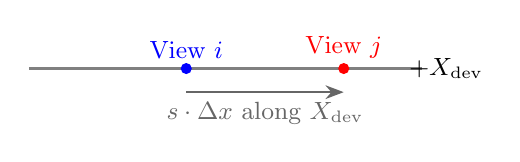
\begin{tikzpicture}[>=Stealth, scale=1.0]
  \draw[gray, thick] (-2,0) -- (3,0);
  \fill[blue] (0,0) circle(2pt) node[above]{\small View $i$};
  \fill[red] (2,0) circle(2pt) node[above]{\small View $j$};
  \draw[->, thick, black!60] (0,-0.3) -- (2,-0.3)
    node[midway, below]{\small $s \cdot \Delta x$ along $X_{\mathrm{dev}}$};
  \node at (3.3,0) {\small $+X_{\mathrm{dev}}$};
\end{tikzpicture}
\end{center}

\medskip
This is the simplest manifold: a \textbf{pure sideways baseline} (like a stereo rig on a slider).
\end{frame}

% ================================================================
\begin{frame}{Linear Rail --- Essential Matrix $E$}
\small
The general Essential matrix formula is:
\vspace{-0.3em}
\[
    E = \skewmat{\mathbf{t}_{ji}} \, R_{ji}
\]
\vspace{-0.8em}
Since $R_{ji} = I$ on a linear rail, this simplifies to:
\vspace{-0.3em}
\[
    E = \skewmat{\mathbf{t}_{\mathrm{cam}}}
\]
\vspace{-0.8em}
The translation in camera coordinates is:
\vspace{-0.3em}
\[
    \mathbf{t}_{\mathrm{cam}} = \Rcd \cdot \mathbf{t}_{\mathrm{dev}}
    = \Rcd \begin{pmatrix} s \\ 0 \\ 0 \end{pmatrix}
\]
\vspace{-0.5em}
Therefore:
\vspace{-0.3em}
\[
    \boxed{E = \skewmat{\Rcd \cdot (s,\; 0,\; 0)^\top}}
\]
\vspace{-0.3em}
\begin{itemize}\setlength{\itemsep}{2pt}
    \item If \texttt{--lin\_allow\_both\_signs} is set, the solver evaluates
          $J(s{=}+1)$ and $J(s{=}-1)$ and picks the best.
    \item Otherwise, $s=+1$ is assumed.
\end{itemize}
\end{frame}

% ================================================================
\section{Sampson Error \& Robust Kernel}
% ================================================================

\begin{frame}{Sampson Distance (First-Order Geometric Error)}
\small
Given calibrated homogeneous points $\hat{\mathbf{x}}_1, \hat{\mathbf{x}}_2 \in \R^3$
and Essential matrix $E$:
\vspace{-0.3em}
\[
    d_{\mathrm{Sampson}}(\hat{\mathbf{x}}_1, \hat{\mathbf{x}}_2, E)
    = \frac{\left(\hat{\mathbf{x}}_2^\top E\, \hat{\mathbf{x}}_1\right)^2}
           {(E\hat{\mathbf{x}}_1)_1^2 + (E\hat{\mathbf{x}}_1)_2^2
          + (E^\top\hat{\mathbf{x}}_2)_1^2 + (E^\top\hat{\mathbf{x}}_2)_2^2}
\]
\vspace{-0.5em}
\begin{itemize}\setlength{\itemsep}{2pt}
    \item This is a \textbf{first-order approximation} to the geometric (reprojection) error.
    \item When $\hat{\mathbf{x}}_2^\top E \hat{\mathbf{x}}_1 = 0$, the point pair
          lies exactly on the epipolar line $\Rightarrow$ zero error.
\end{itemize}

\smallskip
\textbf{Robust Charbonnier kernel} (to downweight outliers):
\vspace{-0.3em}
\[
    \rho(r) = \sqrt{r + \varepsilon^2}, \qquad \varepsilon = 10^{-6}
\]
\vspace{-0.5em}
This is a smooth, differentiable approximation to $\sqrt{r}$ that avoids the
singularity at $r=0$.
\end{frame}

% ================================================================
\section{Match Extraction}
% ================================================================

\begin{frame}{How Matches Are Extracted (\texttt{extract\_xfeat\_matches})}
\small
Given feature maps $F_1, F_2 \in \R^{C \times H \times W}$ and heatmaps $h_1, h_2 \in \R^{H \times W}$:

\begin{enumerate}\setlength{\itemsep}{1pt}
    \item \textbf{Select top-$k$ keypoints} from each heatmap by score.
    \item \textbf{L2-normalize} descriptors at those locations.
    \item Compute $S = D_1 D_2^\top$ (cosine similarity matrix).
    \item \textbf{Mutual nearest neighbor} filter: keep only pairs where
          $\mathrm{NN}_{1\to 2}$ and $\mathrm{NN}_{2\to 1}$ agree.
    \item Discard pairs with $\cos < \texttt{min\_cos}$.
    \item \textbf{Match weight} (NOT detached --- gradients flow!):
\end{enumerate}
\vspace{-0.3em}
\[
    w_m = \frac{\max(\cos_m, 0) \cdot \max(h_1[m], 0) \cdot \max(h_2[m], 0)}
               {\sum_m (\cdots)}
\]
\vspace{-0.5em}
Coordinates are in \textbf{feature-map space} $(x, y)$;
the training loop converts them to \textbf{pixel space} using the stride factor.
\end{frame}

% ================================================================
\section{The Unified Rail Loss}
% ================================================================

\begin{frame}{Rail Loss: Putting It All Together}
\small
Given matches $\{(\mathbf{x}^{(1)}_m, \mathbf{x}^{(2)}_m, w_m)\}_{m=1}^M$ and mode (circular/linear):

\smallskip
\textbf{1. Calibrate points:}
\vspace{-0.3em}
\[
    \hat{\mathbf{x}}^{(k)}_m = K_k^{-1} \begin{pmatrix} u_m \\ v_m \\ 1 \end{pmatrix}
    \quad (k = 0, 1)
\]
\vspace{-0.5em}
\textbf{2. Solve for manifold parameter} (stop-grad):
\begin{itemize}\setlength{\itemsep}{1pt}
    \item Circular: $\phi^* = \arg\min_\phi \; J(\phi)$ \quad (grid + GN)
    \item Linear: $s^* = \arg\min_{s \in \{+1,-1\}} \; J(s)$
\end{itemize}

\textbf{3. Manifold loss} (gradients flow through $w_m$):
\vspace{-0.3em}
\[
    \boxed{J_{\mathrm{manifold}} = \sum_{m} w_m \; \rho\!\bigl(d_{\mathrm{Sampson}}(\hat{\mathbf{x}}^{(1)}_m, \hat{\mathbf{x}}^{(2)}_m, E^*)\bigr)}
\]
\end{frame}

% ================================================================
\begin{frame}{Optional: Deviation Loss $L_{\mathrm{dev}}$}
\small
\textbf{Idea:} Penalize if the manifold fit is much worse than an unconstrained fit.

\smallskip
Compute an unconstrained Essential matrix via \textbf{weighted 8-point algorithm}:
\vspace{-0.3em}
\[
    E_{\mathrm{free}} = \arg\min_E \; \norm{A_w \, \mathrm{vec}(E)}_2^2
    \quad \text{(SVD, projected to Essential manifold)}
\]
\vspace{-0.8em}
\[
    J_{\mathrm{free}} = \sum_m w_m \; \rho\!\bigl(d_{\mathrm{Sampson}}(\hat{\mathbf{x}}^{(1)}_m, \hat{\mathbf{x}}^{(2)}_m, E_{\mathrm{free}})\bigr)
\]
\vspace{-0.8em}
\[
    \boxed{L_{\mathrm{dev}} = \log(J_{\mathrm{manifold}} + \varepsilon) - \log(J_{\mathrm{free}} + \varepsilon)}
\]
\vspace{-0.3em}
\begin{itemize}\setlength{\itemsep}{2pt}
    \item If $L_{\mathrm{dev}} > 0$: manifold fit is worse than free fit
          $\Rightarrow$ matches are inconsistent with the rail.
    \item Weighted by $\lambda_{\mathrm{dev}}$ in the total loss.
\end{itemize}
\end{frame}

% ================================================================
\begin{frame}{Optional: Regularizers}
\small
Two entropy-based regularizers encourage ``healthy'' match distributions:

\smallskip
\textbf{1. Weight entropy} (prevents degenerate weight concentration):
\vspace{-0.3em}
\[
    \mathcal{R}_{\mathrm{entropy}} = -\sum_m p_m \log p_m, \qquad p_m = \frac{w_m}{\sum_j w_j}
\]
\vspace{-0.5em}
\textbf{2. Spatial coverage entropy} (prevents matches clustering in one region):
\begin{itemize}\setlength{\itemsep}{0pt}
    \item Divide image into $B \times B$ bins; accumulate match weights per bin $\rightarrow$ histogram $\mathbf{h}$.
\end{itemize}
\vspace{-0.3em}
\[
    \mathcal{R}_{\mathrm{coverage}} = -\sum_{b=1}^{B^2} q_b \log q_b,
    \qquad q_b = \frac{h_b}{\sum_j h_j}
\]
\vspace{-0.5em}
Both are \textbf{subtracted} from the loss (maximizing entropy = encouraging spread):
\vspace{-0.3em}
\[
    \mathcal{R} = -\lambda_{\mathrm{ent}} \cdot \mathcal{R}_{\mathrm{entropy}}
               - \lambda_{\mathrm{cov}} \cdot \mathcal{R}_{\mathrm{coverage}}
\]
\end{frame}

% ================================================================
\section{Total Loss \& Gradient Flow}
% ================================================================

\begin{frame}{Total Training Loss}
\small
\vspace{-0.3em}
\[
    \boxed{
    \mathcal{L}_{\mathrm{total}} =
        \underbrace{\mathcal{L}_{\mathrm{XFeat}}}_{\text{standard losses}}
      + \lambda_{\mathrm{rail}} \cdot J_{\mathrm{manifold}}
      + \lambda_{\mathrm{dev}} \cdot L_{\mathrm{dev}}
      + \mathcal{R}
    }
\]
\vspace{-0.3em}
\textbf{Standard XFeat losses} (per batch element):
\begin{itemize}\setlength{\itemsep}{1pt}
    \item \textbf{Dual softmax loss} --- coarse descriptor matching (NLL on soft assignment).
    \item \textbf{Coordinate classification loss} --- fine offset prediction (cross-entropy on $8\times 8$ bins).
    \item \textbf{Keypoint position loss} --- distillation from ALIKE keypoints.
    \item \textbf{Keypoint reliability loss} --- heatmap $\leftrightarrow$ confidence alignment.
\end{itemize}

\textbf{Rail losses} (on the fixed image pair):
\begin{itemize}\setlength{\itemsep}{1pt}
    \item $J_{\mathrm{manifold}}$: epipolar consistency on the known manifold.
    \item $L_{\mathrm{dev}}$: deviation from unconstrained fit.
    \item $\mathcal{R}$: entropy regularizers.
\end{itemize}
\end{frame}

% ================================================================
\begin{frame}{Gradient Flow --- What Is Differentiable?}
\small
\begin{center}
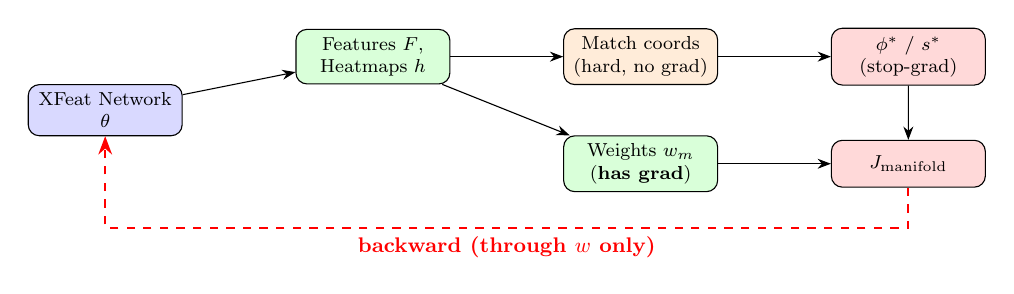
\begin{tikzpicture}[
    box/.style={draw, rounded corners, minimum height=0.7cm, minimum width=2.3cm, align=center, font=\footnotesize},
    >=Stealth, scale=0.85, transform shape
]
\node[box, fill=blue!15] (net) at (0,0) {XFeat Network\\$\theta$};
\node[box, fill=green!15] (feat) at (4,0.8) {Features $F$,\\Heatmaps $h$};
\node[box, fill=orange!15] (match) at (8,0.8) {Match coords\\(hard, no grad)};
\node[box, fill=green!15] (w) at (8,-0.8) {Weights $w_m$\\(\textbf{has grad})};
\node[box, fill=red!15] (solver) at (12,0.8) {$\phi^*$ / $s^*$\\(stop-grad)};
\node[box, fill=red!15] (loss) at (12,-0.8) {$J_{\mathrm{manifold}}$};

\draw[->] (net) -- (feat);
\draw[->] (feat) -- (match);
\draw[->] (feat) -- (w);
\draw[->] (match) -- (solver);
\draw[->] (w) -- (loss);
\draw[->] (solver) -- (loss);
\draw[->, thick, red, dashed] (loss.south) -- ++(0,-0.6) -| (net.south)
    node[pos=0.25, below, font=\small]{\textbf{backward (through $w$ only)}};
\end{tikzpicture}
\end{center}
\vspace{-0.3em}
\begin{itemize}\setlength{\itemsep}{1pt}
    \item \textbf{Match coordinates} selected by \texttt{argmax}/\texttt{topk} --- not differentiable.
    \item \textbf{Match weights} $w_m$ depend on cosine similarity and heatmap values --- \textbf{differentiable}.
    \item Inner solver ($\phi^*$ or $s^*$) wrapped in \texttt{torch.no\_grad()} --- stop-grad.
    \item $\Rightarrow$ Gradients flow through $w_m$ into descriptor and heatmap branches.
\end{itemize}
\end{frame}

% ================================================================
\section{Phase 2: Soft-Assignment Matching}
% ================================================================

\begin{frame}{Phase 2 --- Dual-Softmax Soft Assignment}
\small
\textbf{Phase 1 limitation:} Match coordinates are selected via \texttt{topk}/\texttt{argmax}
--- a \emph{hard}, non-differentiable operation.  Gradients reach the network
only through match \emph{weights} $w_m$.

\smallskip
\textbf{Phase 2 upgrade:} Replace hard selection with a \textbf{dual-softmax soft
assignment} matrix, so match coordinates become \emph{differentiable expectations}:

\vspace{-0.3em}
\[
    P = \mathrm{softmax}\!\bigl(S/\tau,\;\text{dim}=1\bigr)
      \;\odot\;
      \mathrm{softmax}\!\bigl(S/\tau,\;\text{dim}=0\bigr),
    \qquad S = D_1 D_2^\top
\]
\vspace{-0.8em}

For each keypoint $i$ in image 1, the \textbf{soft match coordinate} in image 2 is:
\vspace{-0.3em}
\[
    \tilde{\mathbf{x}}^{(2)}_i = \sum_{j} P_{ij} \; \mathbf{x}^{(2)}_j
    \qquad \text{(weighted average over all candidates)}
\]
\vspace{-0.5em}
\begin{itemize}\setlength{\itemsep}{2pt}
    \item $\tilde{\mathbf{x}}^{(2)}_i$ is differentiable w.r.t.\ descriptors
          $\Rightarrow$ gradients flow through \textbf{both} coordinates \emph{and} weights.
    \item Temperature $\tau$ controls sharpness: low $\tau \to$ nearly hard selection.
    \item \textbf{Stronger learning signal}: the network receives direct feedback on
          \emph{where} it places matches, not just \emph{how much} it trusts them.
\end{itemize}
\end{frame}

% ================================================================
\begin{frame}{Phase 1 vs.\ Phase 2 --- Gradient Flow Comparison}
\small
\begin{columns}[T]
\column{0.48\textwidth}
\begin{center}
\textbf{Phase 1 (current)}\\[0.3em]
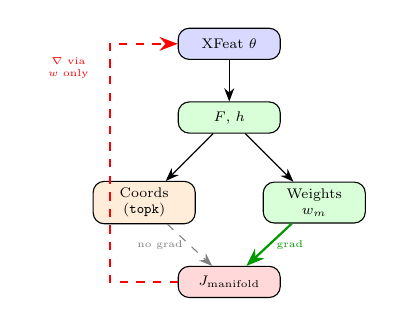
\begin{tikzpicture}[
    box/.style={draw, rounded corners, minimum height=0.55cm, minimum width=1.8cm,
                align=center, font=\scriptsize},
    >=Stealth, scale=0.72, transform shape
]
\node[box, fill=blue!15]   (net1)   at (0, 0)   {XFeat $\theta$};
\node[box, fill=green!15]  (feat1)  at (0,-1.3)  {$F$, $h$};
\node[box, fill=orange!15] (coord1) at (-1.5,-2.8) {Coords\\(\texttt{topk})};
\node[box, fill=green!15]  (w1)     at (1.5,-2.8) {Weights\\$w_m$};
\node[box, fill=red!15]    (loss1)  at (0,-4.2) {$J_{\mathrm{manifold}}$};

\draw[->] (net1)  -- (feat1);
\draw[->] (feat1) -- (coord1);
\draw[->] (feat1) -- (w1);
\draw[->, gray, dashed] (coord1) -- (loss1) node[midway, left, font=\tiny]{no grad};
\draw[->, thick, green!60!black] (w1)  -- (loss1) node[midway, right, font=\tiny]{grad};
\draw[->, thick, red, dashed] (loss1.west) -- ++(-1.2,0) |- (net1.west)
    node[pos=0.45, left, font=\tiny, text width=1.2cm, align=center]{$\nabla$ via\\$w$ only};
\end{tikzpicture}
\end{center}

\column{0.48\textwidth}
\begin{center}
\textbf{Phase 2 (soft assignment)}\\[0.3em]
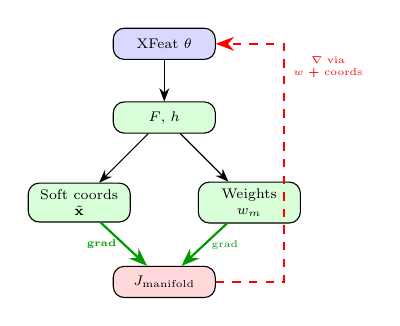
\begin{tikzpicture}[
    box/.style={draw, rounded corners, minimum height=0.55cm, minimum width=1.8cm,
                align=center, font=\scriptsize},
    >=Stealth, scale=0.72, transform shape
]
\node[box, fill=blue!15]   (net2)   at (0, 0)   {XFeat $\theta$};
\node[box, fill=green!15]  (feat2)  at (0,-1.3)  {$F$, $h$};
\node[box, fill=green!15]  (coord2) at (-1.5,-2.8) {Soft coords\\$\tilde{\mathbf{x}}$};
\node[box, fill=green!15]  (w2)     at (1.5,-2.8) {Weights\\$w_m$};
\node[box, fill=red!15]    (loss2)  at (0,-4.2) {$J_{\mathrm{manifold}}$};

\draw[->] (net2)  -- (feat2);
\draw[->] (feat2) -- (coord2);
\draw[->] (feat2) -- (w2);
\draw[->, thick, green!60!black] (coord2) -- (loss2) node[midway, left, font=\tiny]{\textbf{grad}};
\draw[->, thick, green!60!black] (w2)  -- (loss2) node[midway, right, font=\tiny]{grad};
\draw[->, thick, red, dashed] (loss2.east) -- ++(1.2,0) |- (net2.east)
    node[pos=0.45, right, font=\tiny, text width=1.3cm, align=center]{$\nabla$ via\\$w$ \textbf{+} coords};
\end{tikzpicture}
\end{center}
\end{columns}

\vspace{0.5em}
\begin{center}
\small
\begin{tabular}{lcc}
\toprule
& \textbf{Phase 1} & \textbf{Phase 2} \\
\midrule
Match selection        & Hard (\texttt{topk})          & Soft (dual-softmax) \\
Coord differentiable?  & \textcolor{red}{No}           & \textcolor{green!60!black}{\textbf{Yes}} \\
Gradient paths         & Weights only                  & Weights + Coordinates \\
Signal strength        & Indirect                      & Direct \\
\bottomrule
\end{tabular}
\end{center}
\end{frame}

% ================================================================
\section{Summary}
% ================================================================

\begin{frame}{Summary}
\small
\begin{enumerate}\setlength{\itemsep}{2pt}
    \item We augment XFeat training with a \textbf{self-supervision signal} from known
          mechanical motion manifolds.
    \item \textbf{Two manifolds are supported:}
    \begin{itemize}\setlength{\itemsep}{1pt}
        \item \textbf{Circular rail}: device rotates on a circle; 1D parameter $\phi$;
              Essential matrix $E(\phi) = [\mathbf{t}_{ji}]_\times R_{ji}$.
        \item \textbf{Linear rail}: device translates sideways; discrete parameter $s \in \{+1,-1\}$;
              Essential matrix $E = [\Rcd \cdot s\mathbf{e}_1]_\times$.
    \end{itemize}
    \item The loss uses \textbf{Sampson error} with a \textbf{Charbonnier robust kernel}.
    \item \textbf{Phase 1:} Gradients flow through match weights only
          (hard coordinate selection).
    \item \textbf{Phase 2:} Dual-softmax soft assignment makes coordinates differentiable
          $\Rightarrow$ stronger gradient signal through both weights \emph{and} coordinates.
    \item Optional \textbf{deviation loss} and \textbf{entropy regularizers} provide
          additional training signal.
\end{enumerate}

\vspace{0.3em}
\textbf{Result:} The network learns to produce matches that are geometrically consistent
with the deployment manifold, without requiring any labeled data beyond camera calibration.
\end{frame}

% ================================================================
\begin{frame}{}
\begin{center}
    {\Huge Thank You}

    \vspace{1em}
    {\large Questions?}
\end{center}
\end{frame}

\end{document}
